\begin{titre}[Les statistiques]

{\color{bleu3}{\LARGE Calcul de médiane, d'étendue} \hfill{Niveau 3}}
\end{titre}


\begin{CpsCol}
\textbf{Interpréter, représenter et traiter des données}
\begin{description}
\item[$\square$] Calculer une médiane, une étendue
\item[$\square$] Interpréter une caractéristique de position, de dispersion
\end{description}
\end{CpsCol}

\begin{Rec}

Le professeur d'EPS a relevé les performances ci-dessous :
\begin{center}
  \begin{tabularx}{0.85\linewidth}{|l|X|X|l|X|X|}
    \hline
\multicolumn{1}{|c|}{Noms}&Temps au 80~m (s)&Hauteur du saut (cm)&\multicolumn{1}{c|}{Noms}&Temps au 80~m (s)&Hauteur du saut (cm)\\
\hline
Charles&\multicolumn{1}{c|}{13}&\multicolumn{1}{c|}{110}&Gérald&\multicolumn{1}{c|}{13,6}&\multicolumn{1}{c|}{115}\\
Bruno&\multicolumn{1}{c|}{12,5}&\multicolumn{1}{c|}{120}&Nicolas&\multicolumn{1}{c|}{13,9}&\multicolumn{1}{c|}{110}\\
Sylvie&\multicolumn{1}{c|}{15}&\multicolumn{1}{c|}{100}&Florence&\multicolumn{1}{c|}{14,7}&\multicolumn{1}{c|}{110}\\
Brice&\multicolumn{1}{c|}{13,2}&\multicolumn{1}{c|}{125}&Daniel&\multicolumn{1}{c|}{13}&\multicolumn{1}{c|}{125}\\
Carine&\multicolumn{1}{c|}{15,4}&\multicolumn{1}{c|}{100}&Viviane&\multicolumn{1}{c|}{16}&\multicolumn{1}{c|}{95}\\
Léon&\multicolumn{1}{c|}{12}&\multicolumn{1}{c|}{135}&Barbara&\multicolumn{1}{c|}{15,1}&\multicolumn{1}{c|}{105}\\
Christian&\multicolumn{1}{c|}{12,6}&\multicolumn{1}{c|}{130}&Jeanne&\multicolumn{1}{c|}{14,9}&\multicolumn{1}{c|}{110}\\
\'Elisabeth&\multicolumn{1}{c|}{15,4}&\multicolumn{1}{c|}{95}&Lucie&\multicolumn{1}{c|}{15,4}&\multicolumn{1}{c|}{100}\\
Aude&\multicolumn{1}{c|}{14,9}&\multicolumn{1}{c|}{110}&Odile&\multicolumn{1}{c|}{14,2}&\multicolumn{1}{c|}{85}\\
Cécile&\multicolumn{1}{c|}{16,2}&\multicolumn{1}{c|}{85}&Alice&\multicolumn{1}{c|}{15,6}&\multicolumn{1}{c|}{105}\\
Clément&\multicolumn{1}{c|}{12}&\multicolumn{1}{c|}{140}&Gaël&\multicolumn{1}{c|}{13,5}&\multicolumn{1}{c|}{125}\\
Cathy&\multicolumn{1}{c|}{15,8}&\multicolumn{1}{c|}{100}&Pierre&\multicolumn{1}{c|}{12,3}&\multicolumn{1}{c|}{135}\\
Delphine&\multicolumn{1}{c|}{15}&\multicolumn{1}{c|}{105}&Armand&\multicolumn{1}{c|}{12,8}&\multicolumn{1}{c|}{130}\\
Jacques&\multicolumn{1}{c|}{13,1}&\multicolumn{1}{c|}{135}&Jean&\multicolumn{1}{c|}{13,1}&\multicolumn{1}{c|}{115}\\
André&\multicolumn{1}{c|}{13,9}&\multicolumn{1}{c|}{120}&David&\multicolumn{1}{c|}{12,5}&\multicolumn{1}{c|}{135}\\
\hline
  \end{tabularx}
\end{center}
\begin{enumerate}
    \item Quel est le temps en dessous duquel courent 50\% des élèves ?  
    \item Quelle hauteur passent 50\% des élèves ?
\end{enumerate}

\end{Rec}

\begin{DefT}{Médiane}
On appelle Médiane de la série (ou valeur médiane) un nombre qui partage la série en deux groupes de même effectif.
\end{DefT}

\begin{Ex}
On considère la série de notes suivante: $4 ;7 ;8 ;13 ;14 ;15 ;16$.\\
Ici la médiane est $13$ car il y a 3 notes inférieures à $13$ et 3 notes supérieures à $13$.
\end{Ex}

\begin{Mt}
En pratique pour trouver la médiane, on calcule l'effectif total $N$ de la série.
\begin{itemize} 
\item Si $N$ est impair, on choisit la valeur de la série qui occupe le rang $(N+1)\div 2$.
\item Si $N$ est pair, on fait la moyenne entre la valeur de rang  $N\div 2$ et la valeur suivante de la série.
\end{itemize}
\end{Mt}


\begin{Ex} 
\begin{itemize}
\item Si on a 35 valeurs, on calcule $(35+1)\div 2=18$ et la médiane est la $18 \up{ème}$ valeur de la série.
\item Si on a 48 valeurs, on calcule $48\div 2=24$ et la médiane est la moyenne entre la $24 \up{ème}$ valeur et la $25 \up{ème}$ valeur.
\end{itemize}
\end{Ex} 

\begin{AD}

Lors d'un test d'endurance, plusieurs élèves ont eu 12 minutes pour
parcourir la plus grande distance possible. Voici les résultats des
élèves :
2230 -- 2450 -- 1890 -- 1850 -- 2650 -- 2630 -- 2110 -- 2250 -- 2180 --
1980 -- 2000 -- 2850 -- 1950 -- 2920 -- 1975 -- 1910 -- 1860 -- 1930 --
2010 -- 2400 -- 2650 -- 2320 -- 2190 -- 2730 -- 2120 -- 2380 -- 2220.

\begin{enumerate}
\item Calcule la médiane des distances parcourues.
\item Quelle est la distance parcourue par 50\% des élèves ?
\end{enumerate}
\end{AD}

\begin{AD}

\begin{minipage}[top]{10cm}
L'entreprise est à la recherche de qualifications de plus en plus élevées pour faire face au développement de technologies en constante évolution et pour une bonne compréhension des consignes de travail. Lors de sa scolarité, un jeune doit développer de l'intérêt et de la curiosité, si utiles pour réussir ensuite sa vie professionnelle. Face au nombre, en baisse mais encore inquiétant, de sorties du système scolaire sans qualification, il paraît intéressant d'étudier ce phénomène du point de vue européen à la lumière des mathématiques. En France, 13\% des jeunes de 18 à 24 ans qui ne poursuivent pas d'études ni de formation n'ont ni CAP, ni BEP, ni bac et sont sortants précoces.
\end{minipage}
\begin{minipage}{6cm}
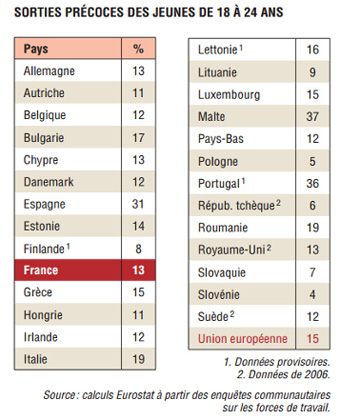
\includegraphics[scale=0.5]{stat12.jpg} 
\end{minipage}

\begin{enumerate}
\item Détermine la médiane des sorties précoces en Europe. 

\item 
\begin{enumerate}
\item Compléter le tableau suivant.

\begin{tabular}{|c|c|c|c|c|c|c|}
\hline 
Sorties précoces en 2007 & [0;5[ & [5;10[ & [10;15[ & [15;20[ & [20;25[ & [25;30] \\ 
\hline 
Effectif de pays européens &  &  &  &  &  &  \\ 
\hline 
E.C.C. des pays européens &  &  &  &  &  &  \\ 
\hline 
\end{tabular} 

\item Construis le polygone des effectifs cumulés croissants.

\item En déduire la médiane des sorties précoces en Europe. 
 
\item Compare avec la question 1.
\end{enumerate}
\end{enumerate}



  
\end{AD}

\begin{DefT}{Etendue}
On appelle \textbf{étendue} d'une série statistique la différence entre la plus grande valeur de la série et la plus petite valeur de la série.
\end{DefT}



\begin{AD}

Lors du devoir commun de Quatrième, voici les résultats de 2 classes.

\begin{minipage}{0.5\linewidth}
\begin{center}
\textbf{Quatrième  1}


\begin{tabular}{|c|c|c|c|c|c|}
\hline 
20 & 18 & 25 & 28& 35 & 27 \\ 
\hline 
22 & 17 & 15 & 26 &37 & 30 \\ 
\hline 
12 & 20 & 21 & 21 & 22 & 30 \\ 
\hline 
30 & 33 & 32 & 23 & 22 & 32 \\ 
\hline 
\end{tabular} 
\end{center}
\end{minipage}
\begin{minipage}{0.5\linewidth}
\begin{center}
\textbf{Quatrième  2}


\begin{tabular}{|c|c|c|c|c|c|}
\hline 
21 & 15 & 25 & 28& 35 & 27 \\ 
\hline 
39 & 9 & 15 & 26 &37 & 30 \\ 
\hline 
15 & 20 & 22 & 21 & 22 & 35 \\ 
\hline 
30 & 30 & 32 & 27 & 29 & 33 \\ 
\hline 
\end{tabular} 
\end{center}
\end{minipage}

\begin{enumerate}
\item Calculer l'étendue de chaque classe.
\item Quelle est la classe la plus hétérogène ?
\item Calculer la médiane de chaque classe.
\item Interpréter les résultats statistiques.
\end{enumerate}
\end{AD}





\begin{autoeval}
\begin{tabular}{p{12cm}p{0.5cm}p{0.5cm}p{0.5cm}p{1cm}}
\textbf{Compétences visées} &  M I & MF & MF  & TBM \vcomp \\ 
Calculer une médiane & $\square$ & $\square$  & $\square$ & $\square$ \\ 
Calculer une étendue & $\square$ & $\square$ & $\square$ & $\square$  \\ 
Interpréter une caractéristique de position& $\square$ & $\square$  & $\square$ & $\square$ \\ 
Interpréter une caractéristique de dispersion & $\square$ & $\square$ & $\square$ & $\square$ \\ 
\end{tabular}
{\footnotesize MI : maitrise insuffisante ; MF = Maitrise fragile ; MS = Maitrise satisfaisante ; TBM = Très bonne maitrise}
 
\end{autoeval}